%----------------------------------------------------------------------------------
% Exemplo do uso da classe beamer para preparar apresentações utilizando LaTeX
% Copyright (C) 2014 PPGCA
% Authors: Diego Antonio Lusa          <diego.antonio.lusa at gmail dot com>
%          Mateus Henrique Dal Forno   <mateush.dalforno at gmail dot com>
%          Rafael Rieder               <rieder at upf dot br>
%----------------------------------------------------------------------------------
\documentclass[t]{beamer}
\usepackage[utf8]{inputenc}
\usepackage{color}
\usepackage[portuguese]{babel}
\usepackage{setspace}
\usepackage{epstopdf}

\title{\textbf{GIT}}
\author{\textbf{Angela Mazzonetto \\ Márcio Nicolau}}
\date{\tiny \today{}}
\institute{\small Universidade de Passo Fundo\\
\centering Programa de Pós-Graduação em Computação Aplicada}
\usetheme{Madrid}

%comandos que alteram a cor do modelo (neste caso para verde)

%\definecolor{fundo}{RGB}{112,20,23} 
\definecolor{fundo}{RGB}{95,17,18} 
%\usecolortheme{fundo}
%\setbeamercolor{title}{bg=black, fg=white}
\setbeamercolor{frametitle}{bg=fundo, fg=white}
\setbeamercolor{block title}{fg=white,bg=fundo}
\setbeamercolor{item projected}{fg=fundo, bg=white}
\setbeamercolor{section in toc}{fg=fundo, bg=white}
%\setbeamercolor{subsection in toc}{fg=fundo}
\setbeamercolor{structure}{fg=fundo}
\setbeamercolor{footline}{fg=white}
\setbeamertemplate{itemize item}[default]
\setbeamertemplate{enumerate item}[default]
%\setbeamertemplate{item projected}[default]
\setbeamertemplate{section in toc}[sections numbered]
%\setbeamertemplate{subsection in toc}[subsections numbered]

% Colocando numero de paginas no slide
\setbeamertemplate{footline} [frame number]

% Desativando os botoes de navegacao
\beamertemplatenavigationsymbolsempty

%inclui a imagem de plano de fundo
{\usebackgroundtemplate{
  \centering
  
\includegraphics[width=\paperwidth]{ppgca.eps}
 }
\begin{document}

\maketitle

\begin{frame} {Tópicos}
\begin{itemize}
\item First steps;
\item Git Essencial;
\item Branching;
\item Tools for GIT.
\end{itemize}
\end{frame}	

\begin{frame} {First steps}
	\begin{itemize}
		\item O que é GIT?
	\end{itemize}
		Git considera que os dados são como um conjunto de snapshots (captura de algo em um determinado instante, como em uma foto) de um mini-sistema de arquivos.

\begin{figure}[tb!]
	\centering
	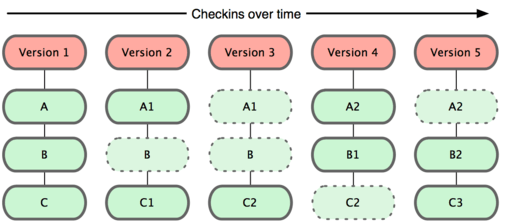
\includegraphics[scale=0.5,keepaspectratio=true]{snapshots.png}
\end{figure}
Figura 1. Git armazena dados como snapshots do projeto ao longo do tempo.	
\end{frame}	

\begin{frame} {First steps}
	\begin{itemize}
  \item Todo o histórico do projeto permanece no disco local;
  \item o Git pode buscar o arquivo de um mês atrás e calcular as diferenças localmente;
  \item há poucas coisas que não possam ser feitas caso esteja offline ou sem acesso a uma VPN;
  \item tudo no Git tem seu checksum (valor para verificação de integridade);
  \item o mecanismo que o Git usa para fazer o checksum é chamado de hash SHA-1:
  	\end{itemize}  	
  		\begin{figure}[tb!]
  			\centering
  			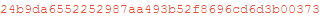
\includegraphics[scale=0.8,keepaspectratio=true]{hash.png}
  		\end{figure}
\end{frame}	

\begin{frame} {First steps}
	\begin{itemize}
		\item Git faz com que seus arquivos sempre estejam em um dos três estados fundamentais: consolidado (committed), modificado (modified) e preparado (staged). 
		\item Dados são ditos consolidados quando estão seguramente armazenados em sua base de dados local. 
		\item Modificado trata de um arquivo que sofreu mudanças mas que ainda não foi consolidado na base de dados.
		\item Um arquivo é tido como preparado quando você marca um arquivo modificado em sua versão corrente para que ele faça parte do snapshot do próximo commit (consolidação).
	\end{itemize}
\end{frame}	

\begin{frame} {First steps}
	\begin{itemize}
		\item Isso nos traz para as três seções principais de um projeto do Git: o diretório do Git (git directory, repository), o diretório de trabalho (working directory), e a área de preparação (staging area).
	\end{itemize}

  		\begin{figure}[tb!]
  			\centering
  			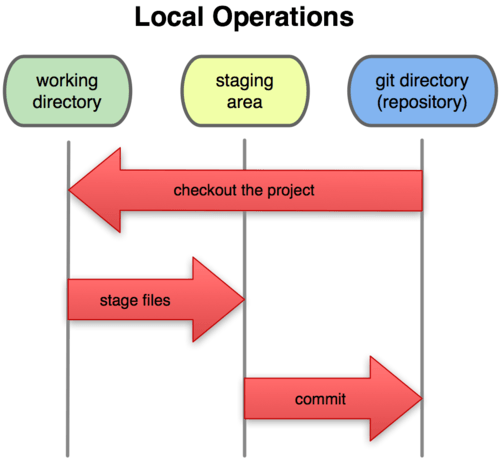
\includegraphics[scale=0.2,keepaspectratio=true]{diretorio.png}
  		\end{figure}
	Figura 1-6. Diretório de trabalho, área de preparação, e o diretório do Git.
	
	
\end{frame}	

\begin{frame} {First steps}
	\begin{itemize}
		\item O workflow básico do Git pode ser descrito assim:
		\begin{itemize}
			\item Você modifica arquivos no seu diretório de trabalho.
			\item Você seleciona os arquivos, adicionando snapshots deles para sua área de preparação.
			\item Você faz um commit, que leva os arquivos como eles estão na sua área de preparação e os armazena permanentemente no seu diretório Git.
		\end{itemize}
	\end{itemize}
\end{frame}
	
\begin{frame} {First steps}
	\begin{itemize}
		\item Instalando e configurando....		
	\end{itemize}
\end{frame}

\begin{frame} {Git Essencial}
	\begin{itemize}
		\item Inicializando um Repositório em um Diretório Existente
		\item Clonando um Repositório Existente
		\item Verificando o Status de Seus Arquivos
		\item Monitorando Novos Arquivos
		\item Selecionando Arquivos Modificados
		\item Ignorando Arquivos
		\item Visualizando Suas Mudanças Selecionadas e Não Selecionadas
		\item Fazendo Commit de Suas Mudanças
		\item Pulando a Área de Seleção
		\item Removendo Arquivos
		\item Movendo Arquivos

	\end{itemize}
\end{frame}

\begin{frame} {Git Essencial}
	\begin{itemize}
		\item Visualizando o Histórico de Commits
		\item Limitando a Saída de Log
		\item Usando Interface Gráfica para Visualizar o Histórico
		\item Modificando Seu Último Commit
		\item Tirando um arquivo da área de seleção
		\item Desfazendo um Arquivo Modificado
		\item Trabalhando com Remotos
		\item Exibindo Seus Remotos
		\item Adicionando Repositórios Remotos
		\item Fazendo o Fetch e Pull de Seus Remotos
		\item Pushing Para Seus Remotos
	\end{itemize}
\end{frame}

\begin{frame} {Git Essencial}
	\begin{itemize}
		\item Inspecionando um Remoto
		\item Removendo e Renomeando Remotos
		\item Tagging		
		\item Listando Suas Tags
		\item Criando Tags
		\item Tags Anotadas
		\item Tags Assinadas
		\item Tags Leves
		\item Verificando Tags
		\item Taggeando Mais Tarde
		\item Compartilhando Tags		
		\item Inspecionando um Remoto
		\item Removendo e Renomeando Remotos

	\end{itemize}
\end{frame}

\begin{frame} {Git Essencial}
	\begin{itemize}
		\item Tagging		
		\item Listando Suas Tags
		\item Criando Tags
		\item Tags Anotadas
		\item Tags Assinadas
		\item Tags Leves
		\item Verificando Tags
		\item Taggeando Mais Tarde
		\item Compartilhando Tags		
		\item Inspecionando um Remoto
		\item Removendo e Renomeando Remotos

	\end{itemize}
\end{frame}

\begin{frame} {Git Essencial}
	\begin{itemize}
		\item Tagging
		\item Listando Suas Tags
		\item Criando Tags
		\item Criando Tags
		\item Tags Anotadas
		\item Tags Assinadas
		\item Tags Leves
		\item Verificando Tags
		\item Taggeando Mais Tarde
		\item Compartilhando Tags
	\end{itemize}
\end{frame}


\begin{frame} {Ramificação (Branching) no Git}
	\begin{itemize}
	\item Criar um branch significa dizer que você vai divergir da linha principal de desenvolvimento e continuar a trabalhar sem bagunçar essa linha principal.
	\item Básico de Branch e Merge
	\item Branch Básico
	\item Merge Básico
	\end{itemize}
	
\end{frame}		
	
\begin{frame} {Git Distribuído - Fluxos de Trabalho Distribuídos}
	\begin{itemize}
		 \item Cada desenvolvedor pode contribuir com código para outros repositórios e ao mesmo tempo pode manter um repositório público em que outros podem basear seu trabalho e que eles podem contribuir. 
		 \item Exemplo Equipe.
	\end{itemize}
	
\end{frame}			
	
\begin{frame} {Ferramentas GIT}
	\begin{itemize}
		\item Git-flow
		\item Source Tree
	\end{itemize}	
\end{frame}		
	
	
\begin{frame} {Fonte:}
		

\begin{figure}[tb!]
	\centering
	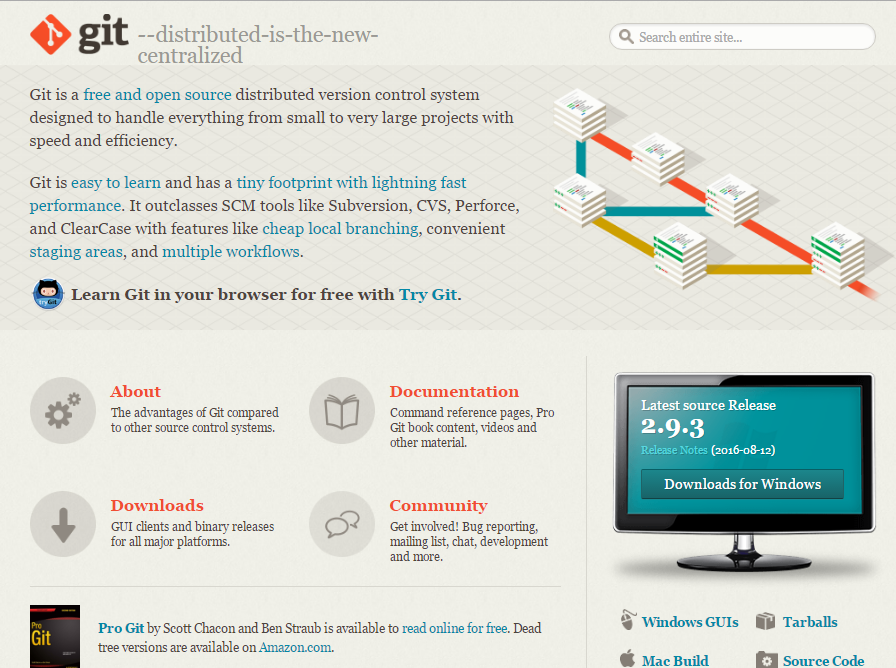
\includegraphics[scale=0.3,keepaspectratio=true]{site.png}
\end{figure}
Figura 1. Livro GIT https://git-scm.com/.	
\end{frame}			

\end{document}
